\chapter{Introduction-How to run this latex template}\label{chapter:introduction}
\section{Required Software}
\textbf{This template was generated with Windows, Linux users might need to double check} 
\begin{itemize}
	\item Install MikTex Console
	\item Install a Tex Editor (TexStudio or the editor of your preference). In this quick tutorial I assume you use TexStudio.
\end{itemize}

\subsection{Linux users}
\begin{itemize}
  \item Install DFKai-SB
  \item Optional: Install \textbf{Times New Roman} font
  \item Make sure you have \textbf{XeLaTeX} installed
  \item Compile with \textbf{XeLaTeX} from the command line
\end{itemize}

\section{Settings in MiKTeX console}
	Before running. Open MikTeX console, and uncheck box shown as follow to make sure MiKTeX console can download packages as required in your document. 
	
	\begin{figure}[ht]                      
		\centering                             
		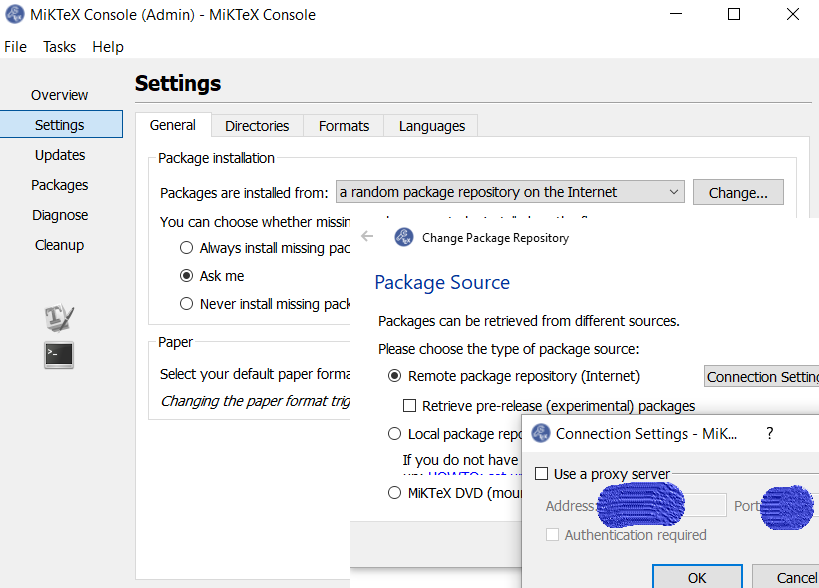
\includegraphics[width = 4in]{figures/UncheckProxyServer.png}
		\caption{Uncheck \textbf{Use proxy server} in MiKTeX console}
		\label{fig:uncheck_proxy_miktex}                         
	\end{figure} 
	Then check for \textbf{Updates} and Install updates in MiKTeX console. Check \textbf{Always install missing packages} or \textbf{Ask me}
\section{Settings in you editor}
Open \textbf{\textit{ThesisTemplate.tex}} with TexStudio.

This template uses the package xeCJK to type chinese characters. This package is not supported with the default compiler PdfLaTeX. Therefor, you need to change your settings to XeLaTeX in your editor. The settings for TexStudio are as follows.

Under Options->Configure TexStudio->Build
\begin{figure}[!h]                      
	\centering                             
	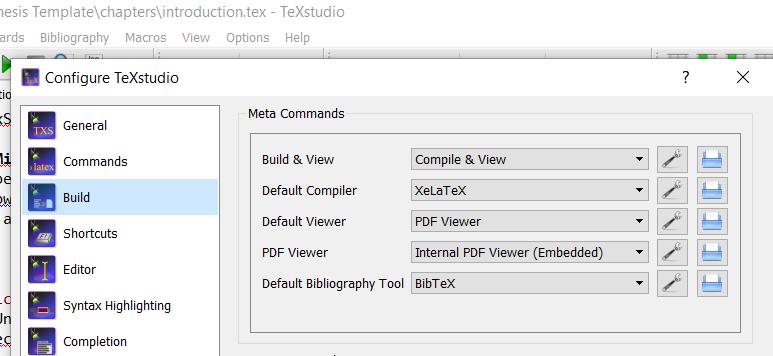
\includegraphics[width = 4in]{figures/TexStudioConfig.png}
	\caption{Set \textbf{XeLaTeX} as default compiler}
	\label{fig:set_xelatex_as_default_compiler}                         
\end{figure}

With all the above settings, if you selected \textbf{Ask me} in MiKTeX console, then the first time you compile TexStudio will as Ask you to install missing packages. Just click  Install. 
\begin{figure}[h]                      
	\centering                             
	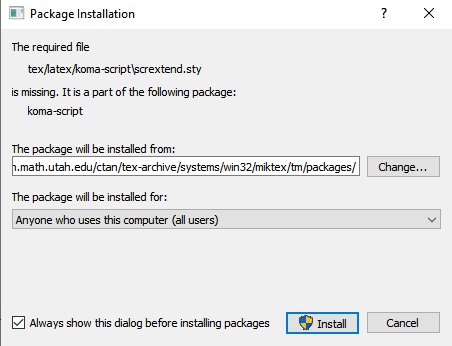
\includegraphics[width = 3in]{figures/InstallMissinPackages.png}
	\caption{TexStudio will automatically select the repository from where the missing package will be downloaded and installed}
	\label{figConquistador}                         
\end{figure} 
